\documentclass{standalone}
\usepackage{tikz}
\begin{document}
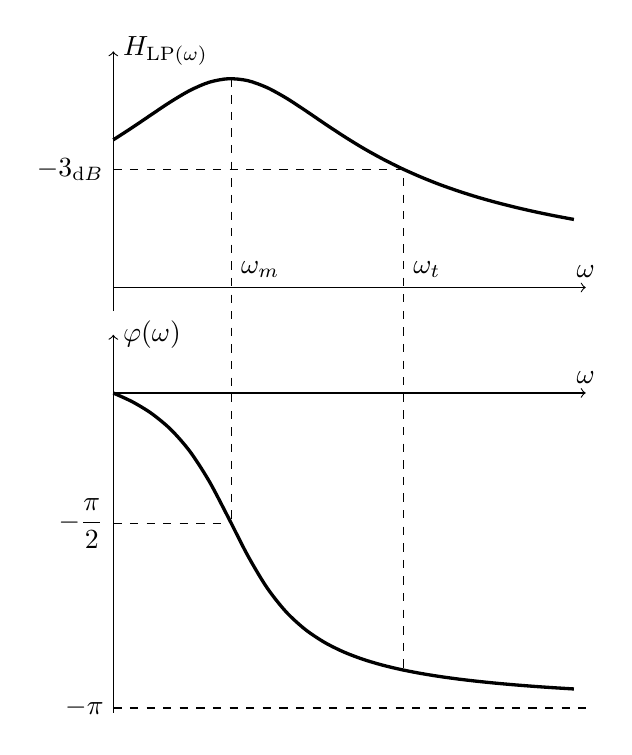
\begin{tikzpicture}[scale=1.5]
    \draw[->](0,1.8)--(0,4)node[right]{$H_{\mathrm{LP}(\omega)}$};
    \draw[->](0,2)--(4,2)node[above]{$\omega$};
    \draw[very thick, smooth, domain=0:3.9]plot(\x,{2+5*((4-2*\x)^2+(2*\x)^2)^(-0.5)});
    \draw[->](0,-1.6)--(0,1.6)node[right]{$\varphi(\omega)$};
    \draw[->](0,1.107)--(4,1.107)node[above]{$\omega$};
    \draw[dashed](0,0)node[left]{$-\displaystyle\frac{\pi}{2}$}--(1,0);
    \draw[dashed](0,-1.56)node[left]{$-\pi$}--(4,-1.56);
    \draw[very thick, smooth, domain=0:3.9]plot(\x,{pi/180*atan(-2*\x+2)});
    \draw[dashed](1,3.768)--(1,2)node[above right]{$\omega_m$}--(1,0);
    \draw[dashed](0,3)node[left]{$-3_{\mathrm{d}B}$}--(2.458,3)--(2.458,2)node[above right]{$\omega_t$}--(2.458,-1.24);
\end{tikzpicture}
\end{document}